\documentclass[10pt,a4paper]{article}

% ---------- geometry ----------
\usepackage[left=1.5cm,right=1.5cm,top=2cm,bottom=1.2cm]{geometry}
\setlength{\parindent}{0pt}
\setlength{\parskip}{4pt plus 1pt}
\pagestyle{plain}

% ---------- fonts ----------
\usepackage[T1]{fontenc}
\usepackage[utf8]{inputenc}
\usepackage{lmodern}
\usepackage{microtype}

% ---------- math ----------
\usepackage{amsmath,amssymb,amsthm}

% ---------- graphics ----------
\usepackage{tikz}
\usetikzlibrary{arrows.meta,positioning,calc,backgrounds,fit,decorations.markings}
\usepackage{tcolorbox}
\tcbuselibrary{skins,breakable}
\usepackage{multicol}

% ---------- colors (Forest Dawn) ----------
\usepackage{xcolor}
\definecolor{accent}{HTML}{1B7A3D}
\definecolor{sky}{HTML}{2D6A4F}
\definecolor{amber}{HTML}{B07D2B}
\definecolor{rose}{HTML}{C0392B}
\definecolor{purple}{HTML}{6B4226}
\definecolor{slate}{HTML}{4A5D4A}
\definecolor{lightbg}{HTML}{ECFDF5}
\definecolor{skybg}{HTML}{F0FFF4}
\definecolor{amberbg}{HTML}{FFFBEB}
\definecolor{rosebg}{HTML}{FFF1F2}
\definecolor{purplebg}{HTML}{FDF4ED}

% ---------- header ----------
\usepackage{fancyhdr}
\pagestyle{fancy}
\fancyhf{}
\renewcommand{\headrulewidth}{0.8pt}
\renewcommand{\headrule}{\hbox to\headwidth{\color{accent}\leaders\hrule height \headrulewidth\hfill}}
\lhead{\small\textbf{CS5100 -- Foundations of Artificial Intelligence}}
\rhead{\small\textbf{Group Seminar Handout}}
\cfoot{\small\thepage}

% ---------- section style ----------
\usepackage{titlesec}
\titleformat{\section}{\Large\bfseries\color{accent}}{}{0em}{}[\vspace{-2pt}]
\titleformat{\subsection}{\large\bfseries\color{sky}}{}{0em}{}
\titleformat{\subsubsection}{\normalsize\bfseries\color{amber}}{}{0em}{}
\titlespacing*{\section}{0pt}{8pt}{3pt}
\titlespacing*{\subsection}{0pt}{6pt}{2pt}
\titlespacing*{\subsubsection}{0pt}{4pt}{1pt}

% ---------- tcolorbox styles ----------
\newtcolorbox{defbox}[1][]{%
  enhanced,colback=skybg,colframe=sky,
  coltitle=white,fonttitle=\bfseries,
  boxrule=0.8pt,arc=4pt,left=6pt,right=6pt,top=4pt,bottom=4pt,
  attach boxed title to top left={yshift=-2mm,xshift=4mm},
  boxed title style={colback=sky,arc=2pt,boxrule=0pt},
  title=#1}

\newtcolorbox{thmbox}[1][]{%
  enhanced,colback=amberbg,colframe=amber,
  coltitle=white,fonttitle=\bfseries,
  boxrule=0.8pt,arc=4pt,left=6pt,right=6pt,top=4pt,bottom=4pt,
  attach boxed title to top left={yshift=-2mm,xshift=4mm},
  boxed title style={colback=amber,arc=2pt,boxrule=0pt},
  title=#1}

\newtcolorbox{algbox}[1][]{%
  enhanced,colback=lightbg,colframe=accent,
  coltitle=white,fonttitle=\bfseries,
  boxrule=0.8pt,arc=4pt,left=6pt,right=6pt,top=4pt,bottom=4pt,
  attach boxed title to top left={yshift=-2mm,xshift=4mm},
  boxed title style={colback=accent,arc=2pt,boxrule=0pt},
  title=#1}

\newtcolorbox{notebox}{%
  enhanced,colback=purplebg,colframe=purple,
  boxrule=0.6pt,arc=3pt,left=6pt,right=6pt,top=3pt,bottom=3pt}

\newtcolorbox{resultbox}{%
  enhanced,colback=rosebg,colframe=rose,
  boxrule=0.8pt,arc=4pt,left=6pt,right=6pt,top=4pt,bottom=4pt}

% ---------- compact lists ----------
\usepackage{enumitem}
\setlist{nosep,leftmargin=14pt,itemsep=2pt}

% ---------- tikz styles for decision trees ----------
\tikzset{
  dtnode/.style={rectangle,rounded corners=3pt,draw=accent,fill=white,
    text=slate,minimum size=16pt,inner sep=3pt,font=\scriptsize\bfseries,
    line width=0.7pt},
  leafyes/.style={circle,draw=accent,fill=accent!15,text=accent,
    minimum size=14pt,inner sep=1pt,font=\scriptsize\bfseries,line width=0.7pt},
  leafno/.style={circle,draw=rose,fill=rose!15,text=rose,
    minimum size=14pt,inner sep=1pt,font=\scriptsize\bfseries,line width=0.7pt},
  dtedge/.style={-{Stealth[length=3pt,width=2.5pt]},semithick,color=slate},
  treebox/.style={draw=slate!30,rounded corners=4pt,fill=lightbg,
    inner sep=4pt,line width=0.5pt},
}

\begin{document}

% ==================== TITLE ====================
\begin{center}
{\LARGE\bfseries\color{accent} The Random Forest Algorithm}\\[3pt]
{\large\color{slate} Ensemble Learning with Decision Trees}\\[2pt]
{\color{slate!60}\rule{0.4\textwidth}{0.4pt}}
\end{center}

% ==================== WHY RANDOM FOREST ====================
\section{Why Random Forest?}

A \textbf{decision tree} is a simple model that learns to ask yes/no questions about data, like a flowchart. We treat it as a \textbf{black box}: feed it data, it automatically learns question rules, and outputs predictions. However, a single tree suffers from \textbf{high variance} --- small changes in training data produce wildly different trees.

Random Forest applies the \textbf{wisdom of crowds}: just as averaging many people's guesses beats any single guess, combining many \textit{diverse} decision trees produces much better predictions than any single tree.

% ==================== DEFINITION ====================
\begin{defbox}[Definition: Random Forest]
A \textbf{Random Forest} is an \textbf{ensemble method} that combines multiple decision trees:
\begin{itemize}
  \item Builds $k$ decision trees, each trained on different data via \textbf{sampling with replacement} (formally called ``bootstrap sampling'')
  \item At each split, considers only $m$ randomly selected features (not all of them), creating diverse trees with different ``perspectives''
  \item Aggregates predictions by \textbf{majority vote} (classification) or \textbf{averaging} (regression)
\end{itemize}
Two sources of randomness --- different \textit{data samples} and different \textit{feature subsets} --- ensure the trees are diverse.
\end{defbox}

\vspace{4pt}

% ==================== ALGORITHM ====================
\begin{algbox}[Random Forest Algorithm]
\begin{enumerate}
  \item \textbf{For} each tree $i = 1, \ldots, k$:
  \begin{enumerate}[label=(\alph*)]
    \item \textbf{Sample data}: Draw $n$ items with replacement from training data (some items appear twice, some are left out)
    \item \textbf{Build tree}: At each node, randomly select $m$ features; split on the best among them
    \item \textbf{Grow fully}: Expand the tree to maximum depth (no pruning)
  \end{enumerate}
  \item \textbf{To predict}: Pass input $\mathbf{x}$ through all $k$ trees, return majority vote:
  $\displaystyle \hat{y} = \text{mode}\bigl\{h_1(\mathbf{x}),\; h_2(\mathbf{x}),\; \ldots,\; h_k(\mathbf{x})\bigr\}$
\end{enumerate}
\end{algbox}

\vspace{4pt}

% ==================== SAMPLING + OOB ====================
\begin{minipage}[t]{0.50\textwidth}
\begin{defbox}[Sampling with Replacement]
Each tree trains on $n$ samples drawn \textit{with replacement}. This means some data points appear multiple times, while others are left out entirely. On average, $\sim63.2\%$ of unique training points are included.

\medskip
\textbf{Probability of being left out:}
\[
P(\text{not picked}) = \left(1 - \frac{1}{n}\right)^n \approx 0.368
\]
\end{defbox}
\end{minipage}\hfill
\begin{minipage}[t]{0.46\textwidth}
\begin{notebox}
\textbf{\color{purple}Free Validation: Out-of-Bag Samples}
\smallskip

The data points that a tree \textit{never saw} during training ($\sim36.8\%$) are called \textbf{out-of-bag (OOB)} samples. We test each tree on its own unseen samples to get a \textbf{free accuracy estimate} --- no separate test set needed!

\smallskip
This is similar in accuracy to $k$-fold cross-validation.
\end{notebox}
\end{minipage}

\newpage

% ==================== PAGE 2: WORKED EXAMPLE ====================
\section{Step-by-Step Example}

Using a hiking dataset with features: \textbf{Outlook}, \textbf{Temperature}, \textbf{Humidity}, \textbf{Wind} $\to$ \textbf{Go Hiking?}

We build a tiny forest: 3 trees, each split considers 2 of 4 features.

\begin{multicols}{2}

\subsubsection{Tree 1\;\; \textcolor{amber}{Outlook \& Wind}}

\textbf{Sampled rows}: \{1,1,3,4,5,7,7,8\}\\
Random features at root: \{Outlook, Wind\}

\begin{center}
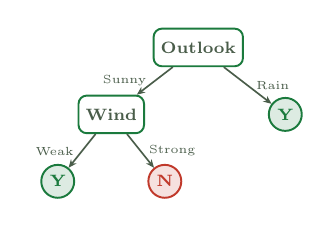
\begin{tikzpicture}[scale=0.85, every node/.style={transform shape}]
  \node[dtnode] (r1) at (0,0) {Outlook};
  \node[dtnode] (w1) at (-1.3,-1) {Wind};
  \node[leafyes] (y1) at (1.3,-1) {Y};
  \node[leafyes] (y2) at (-2.1,-2) {Y};
  \node[leafno]  (n1) at (-0.5,-2) {N};
  \draw[dtedge] (r1) -- node[left,font=\tiny]{Sunny} (w1);
  \draw[dtedge] (r1) -- node[right,font=\tiny]{Rain} (y1);
  \draw[dtedge] (w1) -- node[left,font=\tiny]{Weak} (y2);
  \draw[dtedge] (w1) -- node[right,font=\tiny]{Strong} (n1);
\end{tikzpicture}
\end{center}

\subsubsection{Tree 2\;\; \textcolor{amber}{Humidity \& Temp}}

\textbf{Sampled rows}: \{2,3,3,5,6,6,8,9\}\\
Random features at root: \{Humidity, Temperature\}

\begin{center}
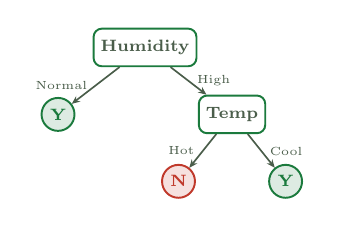
\begin{tikzpicture}[scale=0.85, every node/.style={transform shape}]
  \node[dtnode] (r2) at (0,0) {Humidity};
  \node[leafyes] (y3) at (-1.3,-1) {Y};
  \node[dtnode] (t2) at (1.3,-1) {Temp};
  \node[leafno]  (n2) at (0.5,-2) {N};
  \node[leafyes] (y4) at (2.1,-2) {Y};
  \draw[dtedge] (r2) -- node[left,font=\tiny]{Normal} (y3);
  \draw[dtedge] (r2) -- node[right,font=\tiny]{High} (t2);
  \draw[dtedge] (t2) -- node[left,font=\tiny]{Hot} (n2);
  \draw[dtedge] (t2) -- node[right,font=\tiny]{Cool} (y4);
\end{tikzpicture}
\end{center}

\subsubsection{Tree 3\;\; \textcolor{amber}{Wind \& Humidity}}

\textbf{Sampled rows}: \{1,2,4,4,6,7,9,9\}\\
Random features at root: \{Wind, Humidity\}

\begin{center}
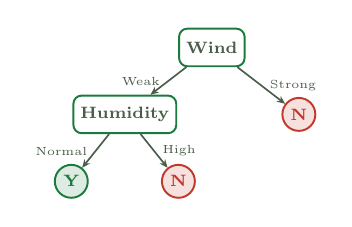
\begin{tikzpicture}[scale=0.85, every node/.style={transform shape}]
  \node[dtnode] (r3) at (0,0) {Wind};
  \node[dtnode] (h3) at (-1.3,-1) {Humidity};
  \node[leafno]  (n3) at (1.3,-1) {N};
  \node[leafyes] (y5) at (-2.1,-2) {Y};
  \node[leafno]  (n4) at (-0.5,-2) {N};
  \draw[dtedge] (r3) -- node[left,font=\tiny]{Weak} (h3);
  \draw[dtedge] (r3) -- node[right,font=\tiny]{Strong} (n3);
  \draw[dtedge] (h3) -- node[left,font=\tiny]{Normal} (y5);
  \draw[dtedge] (h3) -- node[right,font=\tiny]{High} (n4);
\end{tikzpicture}
\end{center}

\columnbreak

\subsubsection{Aggregation: Majority Vote}

\textbf{New data point:}\\
Outlook=Sunny, Temp=Cool, Humidity=Normal, Wind=Weak

\medskip

\renewcommand{\arraystretch}{1.4}
{\small
\begin{tabular}{@{}llc@{}}
\textbf{\color{sky}Tree} & \textbf{Path through tree} & \textbf{Vote}\\
\hline
Tree 1 & Outlook$=$Sunny $\to$ Wind$=$Weak & \textcolor{accent}{\textbf{Yes}}\\
Tree 2 & Humidity$=$Normal & \textcolor{accent}{\textbf{Yes}}\\
Tree 3 & Wind$=$Weak $\to$ Humidity$=$Normal & \textcolor{accent}{\textbf{Yes}}\\
\end{tabular}}

\vspace{6pt}

\begin{resultbox}
\textbf{Final vote: 3--0 in favor of Yes.}\\[2pt]
The Random Forest predicts: \textbf{\color{accent}Yes --- go hiking!}\\[2pt]
{\small Even if one tree had disagreed, majority vote would smooth out the error.}
\end{resultbox}

\vspace{8pt}

% ==================== FEATURE IMPORTANCE ====================
\subsection{Feature Importance}

How do we know which features matter most? Simple test:
\begin{enumerate}
  \item Record the forest's accuracy on unseen (out-of-bag) data
  \item For one feature: randomly \textbf{shuffle} its values, breaking its relationship with the outcome
  \item Re-evaluate accuracy --- if it drops a lot, that feature was important!
  \item Repeat for each feature and rank by drop size
\end{enumerate}
{\small This is called \textbf{permutation importance}. The bigger the accuracy drop, the more the model depends on that feature.}

\end{multicols}

\vspace{4pt}

% ==================== KEY TAKEAWAYS ====================
\begin{center}
\colorbox{lightbg}{\parbox{0.92\textwidth}{\centering
\textbf{\large\color{accent} Key Takeaways}\\[4pt]
\begin{minipage}{0.88\textwidth}
\begin{enumerate}
  \item \textbf{\color{sky}Diversity reduces variance}: Sampling with replacement + random feature selection create diverse trees whose errors cancel out
  \item \textbf{\color{amber}Free validation}: Out-of-bag samples provide a free accuracy estimate --- no separate test set needed
  \item \textbf{\color{purple}Interpretable}: Permutation importance reveals which features drive the model's predictions
\end{enumerate}
\end{minipage}}}
\end{center}

\end{document}
